\documentclass[envcountsect, 10pt, portrait, palatino]{beamer}
\usepackage{verbatim}
\usepackage{amsmath}
\usepackage{color}
\usepackage{listings}
%%%%%%%%%%%%%%%%%%%%%%%%%%%%%%% Beamer packages %%%%%%%%%%%%%%%%%%%%%%%
\usetheme{CambridgeUS}
\usefonttheme[onlylarge]{structurebold}
\setbeamerfont*{frametitle}{size=\normalsize,series=\bfseries}
\setbeamertemplate{navigation symbols}{}

\mode<presentation>{
% XXX without this the number does not appear
%\AtBeginDocument{\def\figurename{{\scshape Figure~\thesection.\thefigure}}}
}
% to number captions
\setbeamertemplate{theorems}[ams style]
\setbeamertemplate{caption}[numbered]
%\setbeamertemplate{theorems}[numbered]
%%%%%%%%%%%%%%%%%%%%%%%%%%%% title slide %%%%%%%%%%%%%%%%%%%%%%%%%%%%%%
\title[]{Applied survival analysis}
\author[Constantin T Yiannoutsos]
{ Constantin T Yiannoutsos, Ph.D.}

\date[]{\today}
\newtheorem{defn}{Definition}[section]
\newtheorem{assu}[defn]{Assumption}
\newcommand{\simdot}{\stackrel{\cdot}{\sim}}
\newcommand{\bfbeta}{{\mbox{\boldmath$\beta$}}}
\newcommand{\bfep}{{\mbox{\boldmath$\epsilon$}}}
\newcommand{\bhat}{\hat{\beta}}
\newcommand{\btilde}{\tilde{\mbox{\boldmath$\beta$}}}
\newcommand{\bfmu}{{\mbox{\boldmath$\mu$}}}
\newcommand{\Var}{{\rm Var}}
\newcommand{\Cov}{{\rm Cov}}
\newcommand{\trt}{{\rm trt}}
\newcommand{\pr}{{\rm pr}}
\newcommand{\age}{{\rm age}}
\newcommand{\Sin}{\sum_{i=1}^N}
\newcommand{\Sjn}{\sum_{j=1}^N}
\newcommand{\ui}{{\bf u}_i}
\newcommand{\uj}{{\bf u}_j}
\newcommand{\bfx}{{\mbox{{\bf x}}}}
\newcommand{\bfp}{{\mbox{{\bf p}}}}
\newcommand{\hbfp}{\widehat{\mbox{{\bf p}}}}
\newcommand{\bfy}{{\mbox{{\bf y}}}}
\newcommand{\bfY}{{\mbox{{\bf Y}}}}
\newcommand{\bfZ}{{\mbox{{\bf Z}}}}
\newcommand{\bfa}{{\mbox{{\bf a}}}}
\newcommand{\bfb}{{\mbox{{\bf b}}}}
\newcommand{\bfg}{{\mbox{{\bf g}}}}
\newcommand{\bfU}{{\bf U}}
\newcommand{\bfu}{{\mbox{{\bf u}}}}
\newcommand{\bfz}{{\mbox{{\bf z}}}}
\newcommand{\logit}{{\mbox{{logit}}}}
\newcommand{\bfzero}{{\mbox{{\bf 0}}}}
\newcommand{\hbeta}{{\widehat \beta}}
\newcommand{\heta}{{\widehat \eta}}
\newcommand{\hsigma}{{\widehat \sigma}}
\newcommand{\hmu}{{\widehat \mu}}
\newcommand{\hpi}{{\widehat \pi}}
\newcommand{\cI}{{\cal I}}
\newcommand{\bsigma}{{\bar \sigma}}
\newcommand{\brho}{{\bar \rho}}
\newcommand{\bx}{ {\bar {x} } }
\newcommand{\bY}{ {\bar {Y} } }
\newcommand{\hY}{ {\widehat {Y} } }
\newcommand{\hp}{ {\widehat {p} } }
\newcommand{\hVar}{ {\widehat {Var} } }

\setlength{\baselineskip}{2.5em}
% The main document
\begin{document}
\begin{frame}
  \titlepage
\end{frame}
%%%%%%%%%%%%%%%%%%%%%%%%%%%%%%%%%%%%%%%%%%%%%%%%%%%%%%%%%%%%%%%%%%%%%%%
\begin{frame}{Contents of today's lecture}
  \tableofcontents
\end{frame}
\section{More on the Cox model}
\subsection{Introduction}
\begin{frame}{More on the Cox PH model}
In today's lecture we will deal with:
\begin{itemize}
\item[I.] Confidence intervals and hypothesis tests
\begin{itemize}
\item Two methods for confidence intervals
\vspace{0.2in}
\item Wald tests and likelihood ratio tests
\vspace{0.2in}
\item Interpretation of parameter estimates
\vspace{0.2in}
\item An example with real data from an AIDS clinical trial
\end{itemize}
\item[II.] Predicted survival under proportional hazards
\item[III.] Predicted medians and P-year survival
\end{itemize}
%%%%%%%%%%%%%%%%%%%%%%%%%%%%%%%%%%%%%%%%%%%%%%%%%%%%%%%%%%%%%%%%%%%%%%%%%%%%
\end{frame}
\subsection{Confidence intervals for the hazard ratio}
\begin{frame}{Constructing Confidence intervals and tests for the Hazard Ratio}
Reference: see Collett 3.4
\\[1ex]

Many software packages provide estimates of $\beta$, but
the hazard ratio (i.e., $\exp(\beta)$) is usually the parameter of
interest.
\\[2ex]
We can use the delta method to get standard errors
for $\exp(\hat{\beta})$:\\
\[Var(\exp(\hat{\beta}))=\exp(2\hat{\beta}) Var(\hat{\beta})\]
\end{frame}
\begin{frame}{Constructing confidence intervals for $\exp(\beta)$}
We have two options: (assuming that $\beta$ is a scalar):
\begin{itemize}
\item[I.] Using $se(\exp{\hat\beta})$ obtained above via the delta method
as $se(\exp{\hat\beta})=\sqrt{[Var(\exp(\hat{\beta}))]}$, calculate
the endpoints as:
\begin{eqnarray*}
[L,U] & = & [e^{\hat\beta} - 1.96 \, se(e^{\hat\beta}),
e^{\hat\beta} + 1.96 \, se(e^{\hat\beta})]
\end{eqnarray*}

\item[II.] Form a confidence interval for $\hat{\beta}$, and then
exponentiate the endpoints.
\begin{eqnarray*}
[L,U] & = & [e^{\hat\beta - 1.96 se(\hat\beta)},
e^{\hat\beta + 1.96 se(\hat\beta)}]
\end{eqnarray*}
\end{itemize}

Method II is preferable since $\hat{\beta}$ converges to a normal
distribution more quickly than $\exp(\hat{\beta})$.
%%%%%%%%%%%%%%%%%%%%%%%%%%%%%%%%%%%%%%%%%%%%%%%%%%%%%%%%%%%%%%%%%%%%%%%%%%%%
\end{frame}
\subsection{Hypothesis testing}
\begin{frame}{Hypothesis Tests:}

For each covariate of interest, the null hypothesis is
\begin{eqnarray*}
H_o: \beta_j=0
\end{eqnarray*}
{ A Wald test}\footnote{\scriptsize The first follows a normal
distribution, and the second follows a $\chi^2$ with 1 df.  {\sc
STATA} gives the $Z$ statistic, while {\sc SAS} gives the $\chi^2_1$
test statistic  (the p-values are also given, and don't depend on
which form, $Z$ or $\chi^2$, is provided)} of the above hypothesis
is constructed as:
\begin{eqnarray*}
Z = \frac{\hat{\beta_j}}{se(\hat{\beta_j})} & ~~~\mbox{or}~~~ &
\chi^2 = \left [ \frac{\hat{\beta_j}}{se(\hat{\beta_j})}\right ]^2
\end{eqnarray*}
\end{frame}
\begin{frame}
The test for $\beta_j=0$ assumes that all other terms in the
model are fixed. If we have a factor $A$ with $a$ levels, then we would
need to construct a $\chi^2$ test with $(a-1)$ df, using a test
statistic based on a quadratic form:
\begin{eqnarray*}
\chi^2_{(a-1)} & = &
\widehat\bfbeta_A' Var(\widehat\bfbeta_A)^{-1} \widehat\bfbeta_A
\end{eqnarray*}

where $\bfbeta_A = (\beta_{2},..., \beta_{a})'$ are the $(a-1)$
coefficients corresponding to $Z_2,...,Z_a$ (or $Z_1,...,Z_{a-1}$,
depending on the reference group).
%%%%%%%%%%%%%%%%%%%%%%%%%%%%%%%%%%%%%%%%%%%%%%%%%%%%%%%%%%%%%%%%%%%%%%%%%%%%
\end{frame}
\begin{frame}{Comparing nested models $\Rightarrow$ Likelihood Ratio Tests}

Suppose there are $(p+q)$ explanatory variables measured:
$$Z_1,\ldots,Z_p,Z_{p+1},\ldots,Z_{p+q}$$
and proportional hazards are assumed.
\\[2ex]
\underline{ Consider the following models:}
\begin{itemize}
\item \underline{\bf Model 1:} (contains only the first $p$ covariates)
$$ \frac{\lambda_i(t,\bfZ)}{\lambda_0(t)} =
\exp(\beta_1 Z_1 + \cdots + \beta_p Z_p)$$
\item \underline{\bf Model 2:} (contains all $(p+q)$ covariates)
$$ \frac{\lambda_i(t,\bfZ)}{\lambda_0(t)} =
\exp(\beta_1 Z_1 + \cdots + \beta_{p+q} Z_{p+q})$$
\end{itemize}
\end{frame}
\begin{frame}{Constructing the likelihood-ratio test}
These are {\em nested} models.  For such nested models, we can construct a {\bf likelihood ratio} test of
$$H_0: \beta_{p+1}=\cdots=\beta_{p+q}=0$$ as:
\begin{eqnarray*}
\chi^2_{LR} & = & -2 \left[\log(\hat{L}(1))- \log(\hat{L}(2))\right]
\end{eqnarray*}

Under $H_o$, this test statistic is approximately distributed as
$\chi^2$ with $q$ df.
%%%%%%%%%%%%%%%%%%%%%%%%%%%%%%%%%%%%%%%%%%%%%%%%%%%%%%%%%%%%%%%%%%%%%%%%%%%%
\end{frame}
\begin{frame}[fragile]{Some examples using the R {\tt coxph} command: The likelihood ratio test}

{\bf Model 1:}
\scriptsize
\begin{verbatim}
coxph(formula = Surv(mactime, macstat) ~ karnof + rif + clari,
    data = mac)

  n= 1177, number of events= 121

           coef exp(coef) se(coef)      z Pr(>|z|)
karnof -0.04485   0.95614  0.01064 -4.217 2.48e-05 ***
rif     0.87197   2.39161  0.23694  3.680 0.000233 ***
clari   0.27557   1.31728  0.25801  1.068 0.285509
---
Signif. codes:  0 ‘***’ 0.001 ‘**’ 0.01 ‘*’ 0.05 ‘.’ 0.1 ‘ ’ 1

       exp(coef) exp(-coef) lower .95 upper .95
karnof    0.9561     1.0459    0.9364    0.9763
rif       2.3916     0.4181    1.5032    3.8051
clari     1.3173     0.7591    0.7944    2.1842

Concordance= 0.649  (se = 0.028 )
Rsquare= 0.027   (max possible= 0.73 )
Likelihood ratio test= 32.02  on 3 df,   p=5.193e-07
Wald test            = 32.29  on 3 df,   p=4.548e-07
Score (logrank) test = 33.16  on 3 df,   p=2.977e-07
\end{verbatim}
%%%%%%%%%%%%%%%%%%%%%%%%%%%%%%%%%%%%%%%%%%%%%%%%%%%%%%%%%%%%%%%%%%%%%%%%%%%%
\end{frame}
\begin{frame}[fragile]{Likelihood-ratio example (cont'd)}

{\bf Model 2:}

\scriptsize
\begin{verbatim}
coxph(formula = Surv(mactime, macstat) ~ karnof + rif + clari + cd4, data = mac)

  n= 1177, number of events= 121

            coef exp(coef)  se(coef)      z Pr(>|z|)
karnof -0.036874  0.963798  0.010665 -3.457 0.000546 ***
rif     0.879749  2.410294  0.237092  3.711 0.000207 ***
clari   0.252345  1.287041  0.258337  0.977 0.328664
cd4    -0.018360  0.981807  0.003684 -4.984 6.23e-07 ***
---
Signif. codes:  0 ‘***’ 0.001 ‘**’ 0.01 ‘*’ 0.05 ‘.’ 0.1 ‘ ’ 1

       exp(coef) exp(-coef) lower .95 upper .95
karnof    0.9638     1.0376    0.9439    0.9842
rif       2.4103     0.4149    1.5145    3.8360
clari     1.2870     0.7770    0.7757    2.1354
cd4       0.9818     1.0185    0.9747    0.9889

Concordance= 0.716  (se = 0.028 )
Rsquare= 0.053   (max possible= 0.73 )
Likelihood ratio test= 63.77  on 4 df,   p=4.682e-13
Wald test            = 55.59  on 4 df,   p=2.449e-11
Score (logrank) test = 56.22  on 4 df,   p=1.806e-11
\end{verbatim}
%%%%%%%%%%%%%%%%%%%%%%%%%%%%%%%%%%%%%%%%%%%%%%%%%%%%%%%%%%%%%%%%%%%%%%%%%%%%
\end{frame}
\begin{frame}[fragile]{The likelihood ratio test of significance for the CD4 count}
The {\bf likelihood ratio} test for the effect of CD4 is 

\begin{eqnarray*}
\chi^2_{LR} & = & -2 \left[\log(\hat{L}(1))- \log(\hat{L}(2))\right]\\
            & = & -2 \left[-754.4910- (-738.6162 ))\right]=31.7496
\end{eqnarray*}
This is compared to a chi-square statistic with 1 degree of freedom, resulting in a p-value which is virtually zero.  The R code and results are as follows:

\small
\begin{verbatim}
Analysis of Deviance Table
 Cox model: response is  Surv(mactime, macstat)
 Model 1: ~ karnof + rif + clari
 Model 2: ~ karnof + rif + clari + cd4
   loglik Chisq Df P(>|Chi|)
1 -754.49
2 -738.62 31.75  1 1.754e-08 ***
---
Signif. codes:  0 ‘***’ 0.001 ‘**’ 0.01 ‘*’ 0.05 ‘.’ 0.1 ‘ ’ 1
\end{verbatim}
\end{frame}
\begin{frame}[fragile]{Estimates of the hazard ratio}
The above output produces the estimated hazard
ratio along with 95\% confidence intervals by forming a CI for the log HR (beta), 
and then exponentiating the bounds)
\\[2ex]
We can also compute the hazard ratio ourselves, by
exponentiating the coefficients:
\begin{eqnarray*}
HR_{cd4} & = & \exp(-0.01835) = 0.98
\end{eqnarray*}
... or with R, 

\small
\begin{verbatim}
exp(confint(fit.mac1))
           2.5 %    97.5 %
karnof 0.9438599 0.9841573
rif    1.5144570 3.8360410
clari  0.7757030 2.1354482
cd4    0.9747439 0.9889221
\end{verbatim}

Why is this HR so close to 1, and yet still significant?
\end{frame}
\begin{frame}[fragile]{What is the interpretation of this HR?}
\end{frame}
\subsection{Carrying out custom tests}
\begin{frame}[fragile]{Comparison of treatment effect for MAC}
In the mac study, there were three treatment arms (rif,
clari, and the rif+clari combination).  Because we have only included
the {\tt rif} and {\tt clari} effects in the model, the combination
therapy is the ``reference'' group.
\\[2ex]
We can conduct an overall test of treatment using the {\tt wald.test}
command in R (part of the {\tt aod} package):

\small
\begin{verbatim}
Wald test:
----------

Chi-squared test:
X2 = 17.0, df = 2, P(> X2) = 2e-04
\end{verbatim}
\normalsize
for a 2 df Wald chi-square test of whether both treatment
coefficients are equal to 0.  This {\tt wald.test} command can
be used to conduct many diffferent tests based on the Wald test.
\end{frame}
\begin{frame}[fragile]{Testing the difference between treatment arms}
We can also test whether there is
a difference between the {\tt rif} and {\tt clari} treatment arms:

\scriptsize
\begin{verbatim}
Call:
coxph(formula = Surv(mactime, macstat) ~ karnof + rif + I(rif +
    clari) + cd4, data = mac)

  n= 1177, number of events= 121

                    coef exp(coef)  se(coef)      z Pr(>|z|)
karnof         -0.036874  0.963798  0.010665 -3.457 0.000546 ***
rif             0.627403  1.872742  0.211970  2.960 0.003078 **
I(rif + clari)  0.252345  1.287041  0.258337  0.977 0.328664
cd4            -0.018360  0.981807  0.003684 -4.984 6.23e-07 ***
---
Signif. codes:  0 ‘***’ 0.001 ‘**’ 0.01 ‘*’ 0.05 ‘.’ 0.1 ‘ ’ 1
\end{verbatim}
\normalsize
Here the test of the difference between the two arms is $\chi^2=2.960$ with p-value $p=0.0031$.
\end{frame}
\begin{frame}[fragile]{Testing the difference between treatment arms (cont'd)}
In the above, the factor {\tt rif} summarizes the combined effect of rifabutin and clarithromycin, while the factor {I(rif+clar)} evaluates the sum of the two\footnote{Note that the function ``{\tt I()} means ``as is", that is, it asks R to produce the sum of the factors and not interpret the ``+" as part of the formula.}
\\[2ex]
This can also be done explicitly by the Wald test by defining a contrast matrix $L=\{0,-1,1,0\}$ (since the coefficients for {\tt rif} and {\tt clar} are, respectively, second and third in the coefficient matrix $b$) by a Wald test\footnote{Note that the Wald chi-square statistic is $\chi^2_{Wald}=z_{Wald}^2=(2.960)^2=8.8$.}

\small
\begin{verbatim}
Wald test:
----------

Chi-squared test:
X2 = 8.8, df = 1, P(> X2) = 0.0031
\end{verbatim}
\end{frame}

\section{Predicted survival in the Cox model}
\subsection{Introduction}
\begin{frame}{Predicting survival through the Cox model}
The major drawback of the Cox model is that it does not provide estimates for $\lambda_0(t)$ the baseline hazard.\\[2ex]
The Cox PH model says that
$\lambda_i(t,\bfZ)=\lambda_0(t) \,\exp(\bfbeta \bfZ)$.
What does this imply about the survival function, $S_z(t)$, for
the i-th individual with covariates $\bfZ_i$?
\\[2ex]
For the baseline (reference) group, we have:
\begin{eqnarray*}
S_0(t) & = & e^{- \int_0^t \lambda_0(u) du} = e^{-\Lambda_0(t)}
\end{eqnarray*}

This is by the definition of a survival function (see intro notes).

\end{frame}
\begin{frame}{Without estimating $\lambda_0(t)$ we cannot estimate $S(t;\bfZ)$}
For the $i$-th patient with covariates $\bfZ_i$, we have:

\vspace{-0.3in}
\
\begin{eqnarray*}
S_i(t) & = & e^{- \int_0^t \lambda_i(u) du} = e^{-\Lambda_i(t)}
\nonumber \\[1ex]
       & = & e^{- \int_0^t \lambda_0(u) \exp(\bfbeta \bfZ_i) du}
\nonumber \\[1ex]
       & = & e^{- \exp(\bfbeta \bfZ_i) \int_0^t \lambda_0(u) du}
\nonumber  \\[1ex]
       & = & \left[e^{- \int_0^t \lambda_0(u) du}\right]^{\exp(\bfbeta\bfZ_i)}
\nonumber \\[1ex]
       & = & \left[S_0(t)\right]^{\exp(\bfbeta\bfZ_i)}
\end{eqnarray*}
(This uses the mathematical relationship $[e^b]^a = e^{ab}$)\\[2ex]
Thus, if we cannot estimate $\lambda_0(t)$ we cannot estimate $S_0(t)$ and, consequently, we cannot estimate $S(t;\bfZ)$.
%%%%%%%%%%%%%%%%%%%%%%%%%%%%%%%%%%%%%%%%%%%%%%%%%%%%%%%%%%%%%%%%%%%%%%%%%%%%
\end{frame}

\begin{frame}{Estimating $S_0(t)$ through Kaplan Meier}
We could use the KM estimator, but there are a few disadvantages of that approach:
\begin{itemize}
\item It would only use the survival times for observations contained
in the reference group, and not all the rest of the survival times.
\item It would tend to be somewhat choppy, since it would reflect
the smaller sample size of the reference group.
\item It's possible that there are no subjects in the dataset who
are in the ``reference'' group \\[2ex]
For example, say covariates are {\tt health} and {\tt gender};
there is no one of {\tt health}==0 (patients of perfect health) in our dataset.
\end{itemize}
%%%%%%%%%%%%%%%%%%%%%%%%%%%%%%%%%%%%%%%%%%%%%%%%%%%%%%%%%%%%%%%%%%%%%%%%%%%%
\end{frame}
\subsection{Using the Cox model to obtain predicted survival}
\begin{frame}{Taking advantage of the Cox model itself}
Instead, we will use a baseline hazard estimator which
takes advantage of the proportional hazards assumption to get a
smoother estimate.

\begin{eqnarray*}
\hat{S}_i(t) & = & [\hat{S}_0(t)]^{\exp(\widehat\bfbeta\bfZ_i)}
\end{eqnarray*}
Using the above formula, we substitute $\widehat\bfbeta$ based on
fitting the Cox PH model, and calculate $\hat{S}_0(t)$ by
one of the following approaches:
\begin{itemize}
\item Breslow estimator (Stata, R)
\item Kalbfleisch/Prentice estimator (SAS)
\end{itemize}
%%%%%%%%%%%%%%%%%%%%%%%%%%%%%%%%%%%%%%%%%%%%%%%%%%%%%%%%%%%%%%%%%%%%%%%%%%%%
\end{frame}

\subsubsection{The Breslow estimator}
\begin{frame}{The Breslow Estimator}
The Breslow estimator is as follows:
\[ \hat{S}_0(t) = \exp^{-\hat{\Lambda}_0(t)} \]

where $\hat{\Lambda}_0(t)$ is the estimated cumulative baseline hazard:
\[   \hat{\Lambda}(t)  =\sum_{j: \tau_j < t} \left( \frac{d_j}
           {\sum_{k\in {\cal R}(\tau_j)}
      \exp(\beta_1 Z_{1k} + \dots \beta_p Z_{pk})} \right)
\]
\end{frame}
\begin{frame}{The Breslow Estimator:  further motivation}

The Breslow estimator is based on extending the concept of
the Nelson-Aalen estimator to the proportional hazards model.
\\[2ex]
Recall that for a single sample with no covariates, the
{\bf Nelson-Aalen Estimator} of the cumulative hazard is:
\[ \hat{\Lambda}(t)  =\sum_{j: \tau_j < t} \frac{d_j}{r_j} \]
where $d_j$ and $r_j$ are the number of deaths and the
number at risk, respectively, at the $j$-th death time.
\\[2ex]
When there are covariates and assuming the PH model above, one
can generalize this to estimate the cumulative baseline hazard
by adjusting the denominator:
\[ \hat{\Lambda}(t)  =\sum_{j: \tau_j < t} \left( \frac{d_j}
           {\sum_{k\in {\cal R}(\tau_j)}
      \exp(\beta_1 Z_{1k} + \dots \beta_p Z_{pk})} \right)
\]
\end{frame}

\begin{frame}{Heuristic development} 
The expected number of failures in $(t,t+\delta t)$ is
\[ d_j \approx \delta t \times \sum_{k\in {\cal R}(t)} \lambda_0(t)
exp(z_k\hat{\beta}) \]
Hence,
\[ \delta t \times  \lambda_0(t_j) \approx \frac{d_j}{\sum_{k\in {\cal R}(t)}
  exp(z_k\hat{\beta})}     \]
%%%%%%%%%%%%%%%%%%%%%%%%%%%%%%%%%%%%%%%%%%%%%%%%%%%%%%%%%%%%%%%%%%%%%%%%%%%%
\end{frame}
\subsubsection{The Kalbfleisch/Prentice estimator}
\begin{frame}{The Kalbfleisch/Prentice Estimator}
This estimator is as follows:
\[ \hat{S}_0(t) = \prod_{j: \tau_j < t} \hat{\alpha}_j   \]
where $\hat{\alpha}_j, j=1,...d$ are the MLE's obtained by assuming
that $S(t;Z)$ satisfies
\[ S(t;Z) =  [S_0(t)]^{e^{\beta Z}}  =
\left[\prod_{j: \tau_j < t} \alpha_j\right]^{e^{\beta Z}}
= \prod_{j: \tau_j < t} \alpha_j^{e^{\beta Z}} \]

%%%%%%%%%%%%%%%%%%%%%%%%%%%%%%%%%%%%%%%%%%%%%%%%%%%%%%%%%%%%%%%%%%%%%%%%%%%%
\end{frame}

\begin{frame}{ Kalbfleisch/Prentice Estimator: further motivation}

This method is analogous to the Kaplan-Meier Estimator.
Consider  a discrete time model with hazard $(1-\alpha_j)$
at the $j$-th observed death time.

( Note:  we use $\alpha_j=(1-\lambda_j)$ to simplify
the algebra!)

~\\[2ex]
Thus, for someone with z=0, the survivorship function is
\[ S_0(t) = \prod_{j: \tau_j < t} \alpha_j   \]

and for someone with $Z\neq0$, it is:
\[ S(t;Z) =  S_0(t)^{e^{\beta Z}} =
\left[\prod_{j: \tau_j < t} \alpha_j\right]^{e^{\beta Z}}
= \prod_{j: \tau_j < t} \alpha_j^{e^{\beta Z}} \]

\end{frame}
\begin{frame}
The likelihood contributions under this model are:

\begin{itemize}
\item for someone censored at $t$: ~~~ $ S(t;Z)$
\item for someone who fails at $t_j$:~~~
\[ S(t_{(j-1)};Z) -   S(t_j;Z) = \left[ \prod_{k < j}
        \alpha_j \right]^{e^{\beta z}}  [1 - \alpha_j^{e^{\beta Z}}] \]
\end{itemize}

The solution for $\alpha_j$ satisfies:
\[  \sum_{k \in {\cal D}_j} \frac{\exp(Z_k \beta)}{1 -
\alpha_j^{\exp(Z_k \beta)}}
            =  \sum_{k \in {\cal R}_j} \exp(Z_k \beta)  \]

(Note what happens when $Z=0$)
%%%%%%%%%%%%%%%%%%%%%%%%%%%%%%%%%%%%%%%%%%%%%%%%%%%%%%%%%%%%%%%%%%%%%%%%%%%%
\end{frame}
\subsection{Computer implementation}
\begin{frame}{ Obtaining $\hat{S}(t)$ from software packages}
\begin{itemize}
\item  Stata provide the Breslow estimator of $S_0(t;Z)$, but
not predicted survivals at specified covariate values..... you
have to construct these yourself
\item  SAS uses the Kalbfleisch/Prentice estimator of the
baseline hazard, and can provide estimates of survival at
arbitrary values of the covariates with a little bit of
programming.
\item R uses the {\tt coxph} object within the {\tt survfit} command to produce an estimate
of $S(t;Z)$. 
\end{itemize}

In practice, the two methods are {\bf incredibly} close! (see  Fleming and
Harrington 1984, {\em Communications in Statistics}
%%%%%%%%%%%%%%%%%%%%%%%%%%%%%%%%%%%%%%%%%%%%%%%%%%%%%%%%%%%%%%%%%%%%%%%%%%%%
\end{frame}
\begin{frame}[fragile]{Using R to Predict Survival}
Consider predicted survival for the groups of men and women with the best ({\tt health}=2) and worst health ({\tt health}=4). 
The R command {\tt survfit} calculates the predicted survival values.

\scriptsize
\begin{verbatim}
               1          2         3          4
  [1,] 0.9896288 0.98298849 0.9860573 0.97715684    1
  [2,] 0.9815838 0.96987163 0.9752767 0.95963670    2
  [3,] 0.9773101 0.96293165 0.9695622 0.95040011    3
  [4,] 0.9692168 0.94984305 0.9587642 0.93304299    4
  [5,] 0.9587077 0.93295246 0.9447896 0.91076637    5
  [6,] 0.9515173 0.92146452 0.9352587 0.89569475    6
  [7,] 0.9428590 0.90770541 0.9238150 0.87772909    7
   .    .         .          .         .            .
   .    .         .          .         .            .
   .    .         .          .         .            .
[592,] 0.2408962 0.09607878 0.1470458 0.04263921 1088
[593,] 0.2408962 0.09607878 0.1470458 0.04263921 1091
[594,] 0.2408962 0.09607878 0.1470458 0.04263921 1092
\end{verbatim}
\normalsize
In the output above, 1-4 represent the four groups and the last column the 594 distinct failure times when the survival is estimated.
%%%%%%%%%%%%%%%%%%%%%%%%%%%%%%%%%%%%%%%%%%%%%%%%%%%%%%%%%%%%%%%%%%%%%%%%%%%%
\end{frame}
\begin{frame}{Pictorial representation of predicted survival}
We can get a visual picture of what the proportional
hazards assumption implies by looking at these four subgroups.

\centerline{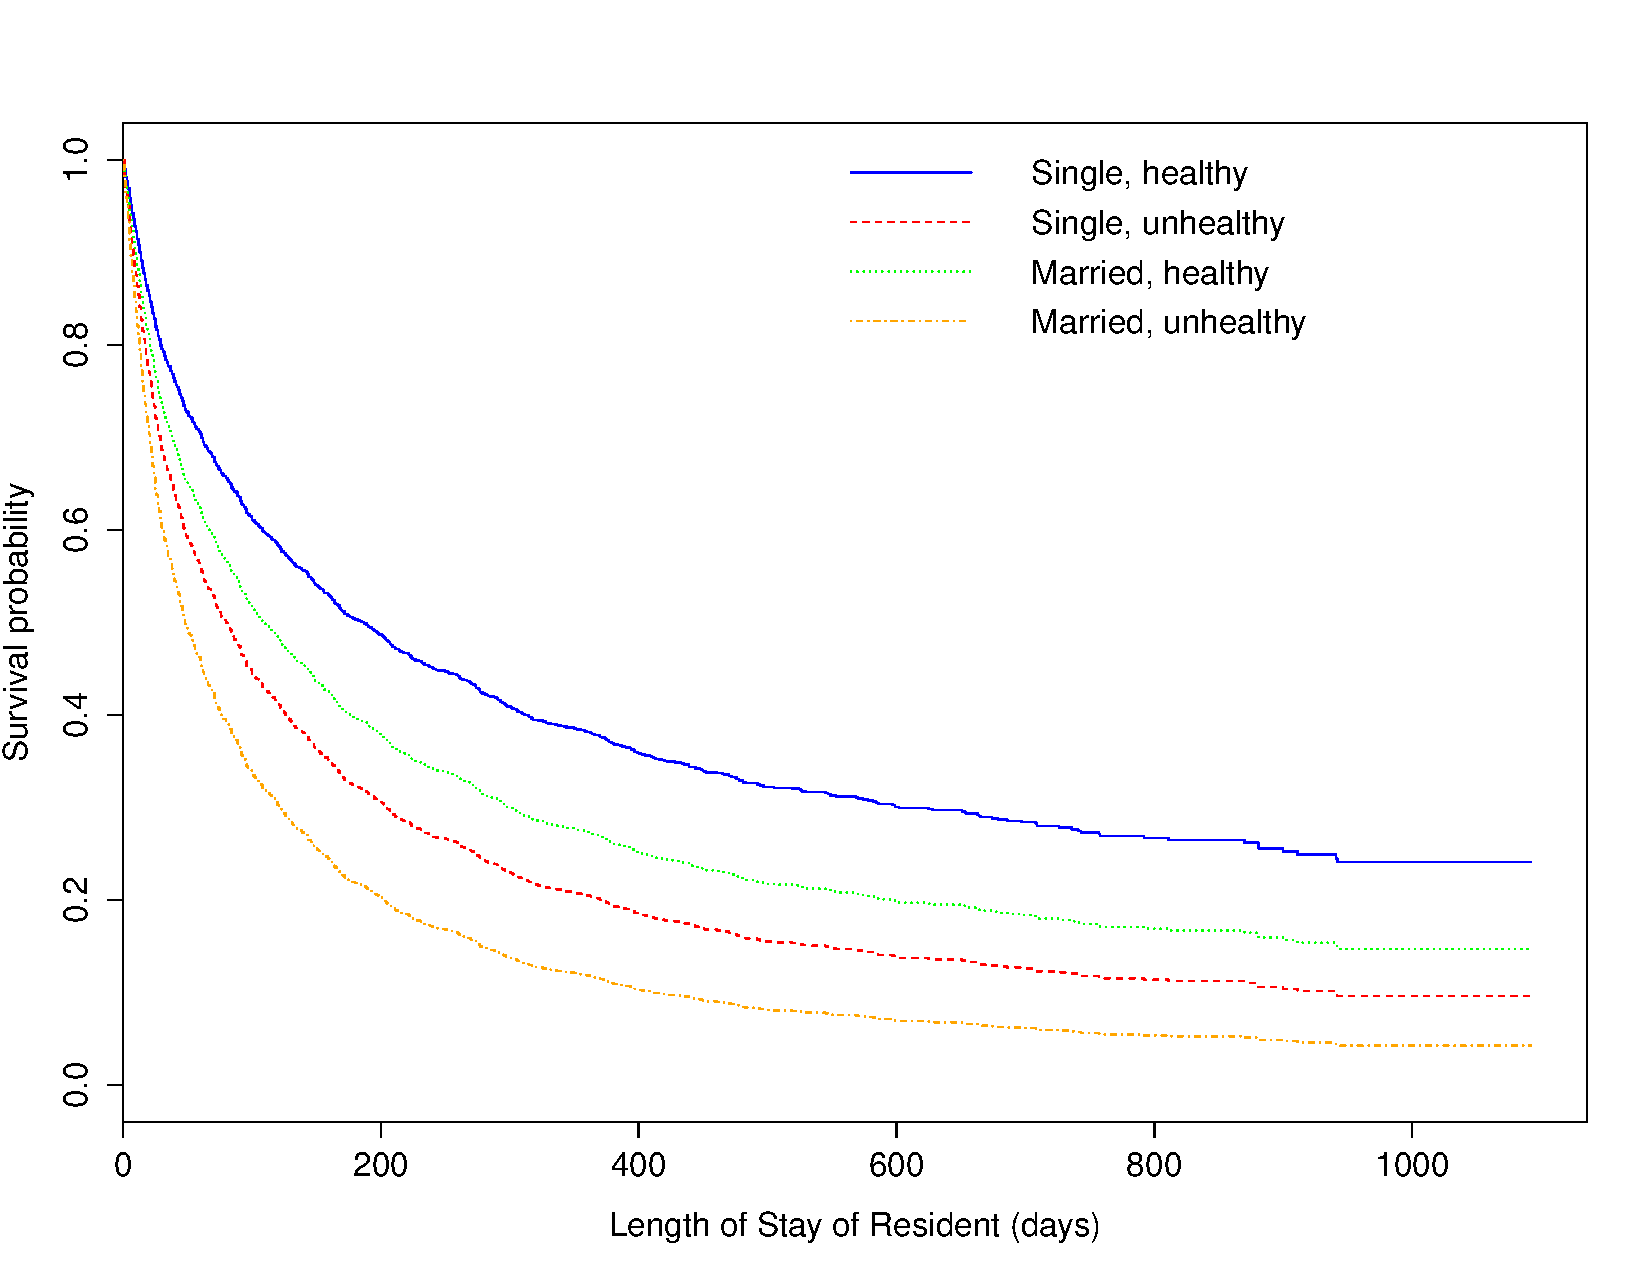
\includegraphics[width=3.5in]{nhpredsurv.pdf}}
\vspace{0.5in}
\end{frame}
%%%%%%%%%%%%%%%%%%%%%%%%%%%%%%%%%%%%%%%%%%%%%%%%%%%%%%%%%%%%%%%%%%%%%%%%%%%%
\begin{frame}[fragile]{Using R to predict survival for subgroups outside the analysis dataset}
We can estimate survival (i.e., $\hat{S}(t;\bfZ)$) even for groups which are not included in the data.\\[2ex]
This is possible because, once we estimate $\hat{S}_0(t)$, the baseline survival, the survival of a group with measurements $\bfZ$ is equal to $\hat{S}(t;\bfZ)=\left [ \hat{S}_0(t)\right ]^{\exp(\bfbeta'\bfZ)}$.
\\[2ex]
This is accomplished in R by creating a new data set with the values of $\bfZ$ as follows:

\small
\begin{verbatim}
newdata2 = data.frame(married = c(0,0,1,1),health = c(0, 2, 0 ,2))
surv.cox2 = survfit(fit.cox, newdata = newdata2)
\end{verbatim}
\end{frame}

\begin{frame}{Calculating the survival of males and females in perfect health}
We can get a visual picture of what the proportional
hazards assumption implies for these four subgroups.
\vspace*{-1in}
\centerline{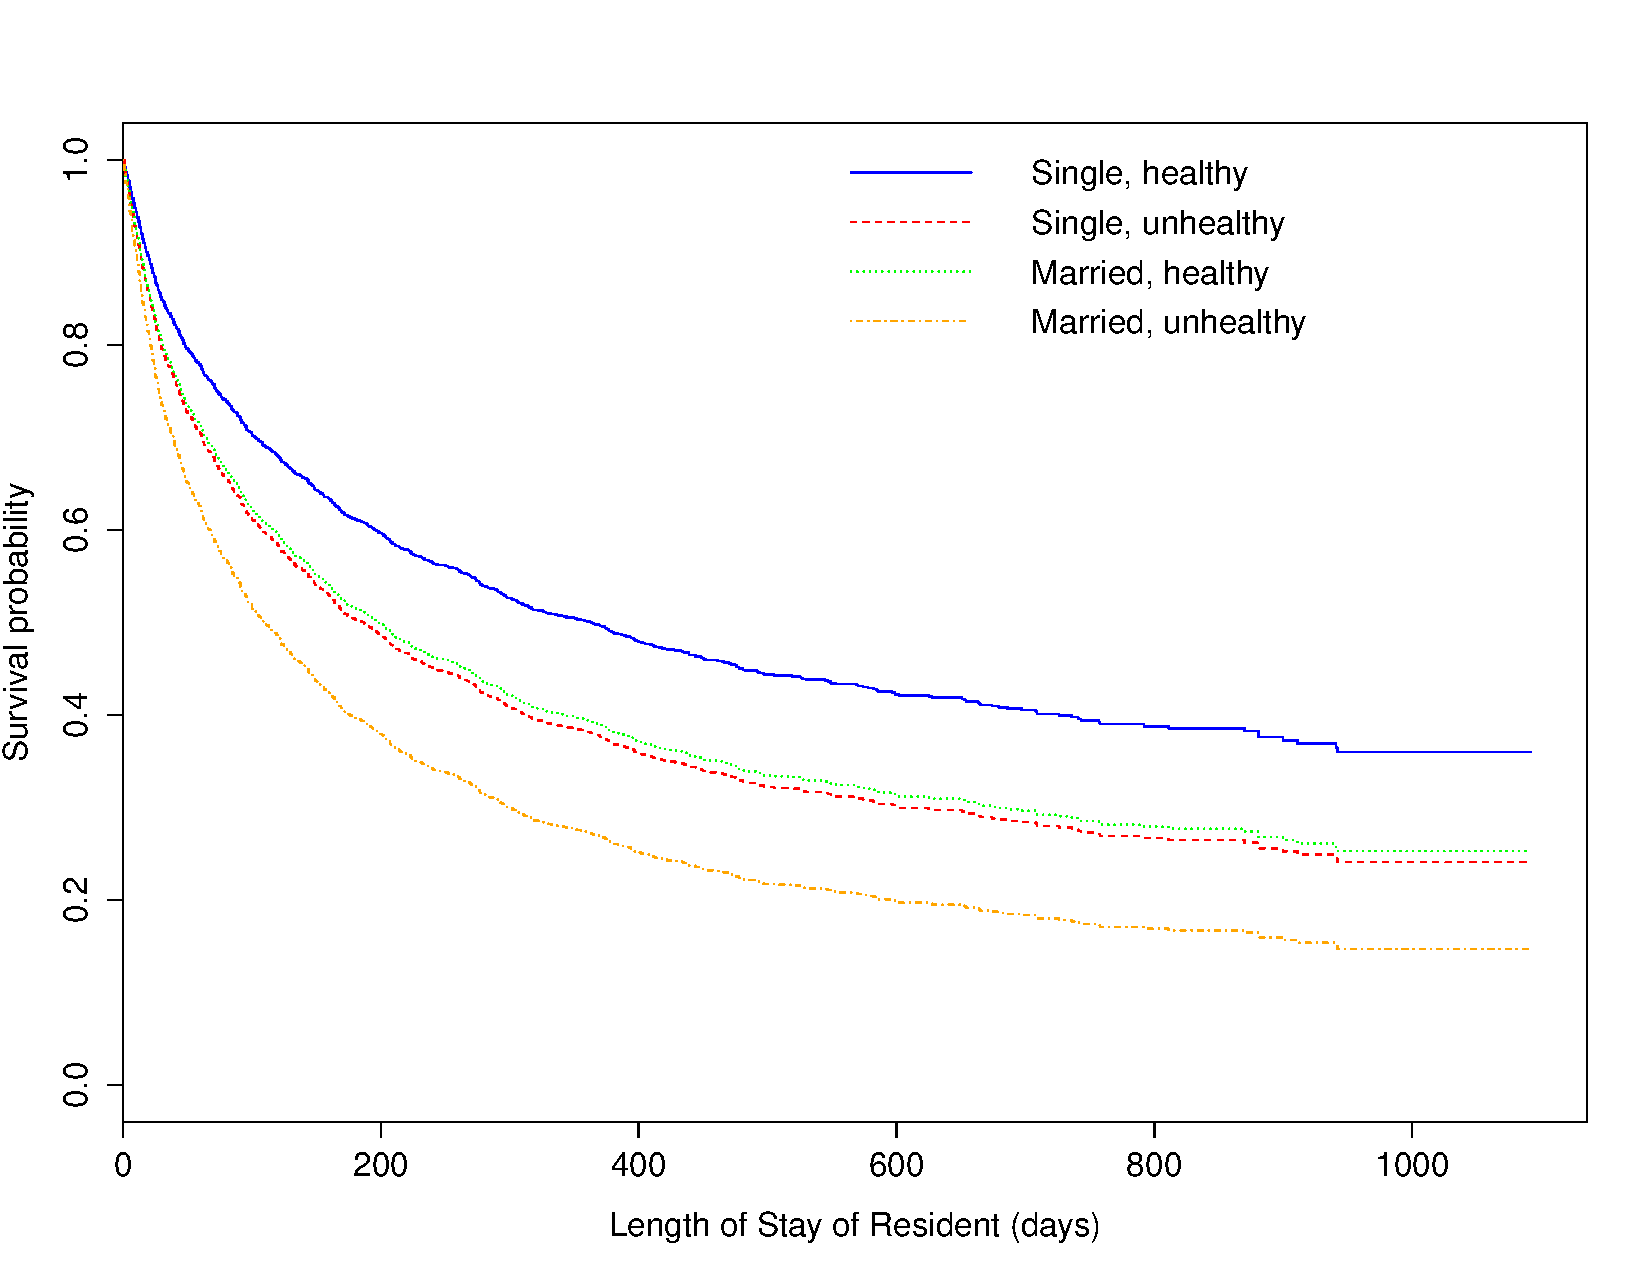
\includegraphics[width=3.5in]{nhpredsurv2.pdf}}
\vspace*{1in}
\end{frame}
%%%%%%%%%%%%%%%%%%%%%%%%%%%%%%%%%%%%%%%%%%%%%%%%%%%%%%%%%%%%%%%%%%%%%%%%%%%%

\subsection{Predicted medians and $P$-year survival}
\subsubsection{Predicting medians}
\begin{frame}{Predicted Medians}
Suppose we want to find the predicted median survival for an
individual with a specified combination of covariates
(e.g., a single male with health status 0 - note that none such individual exists in the data!).\\[2ex]
There are three possible approaches:
\begin{itemize}
\item[(1)] Calculate the median from the subset of individuals with the
specified covariate combination (using KM approach)
\item[(2)] Generate predicted survival curves for each combination of
\item[(3)] Generate the predicted survival curve from the estimated
baseline hazard.  This is done as follows:\\
We want the estimated median ($M$) for an individual with
covariates ${\bfZ_i}$.  We know
\[ S(M;Z) =  [S_0(M)]^{e^{\beta Z_i}}  = 0.5   \]

Hence, $M$ satisfies (multiplying both sides by $e^{-\beta Z_i}$):
\[  S_0(M)  = [0.5]^{e^{-\beta Z_i}}  \]
covariates, and obtain the medians directly.
\end{itemize}
\end{frame}

\begin{frame}[fragile]{Predicting median survival by Kaplan Meier}
Consider the following output:

\scriptsize
\begin{verbatim}
             [,1] [,2]
  [1,] 0.97658863    1
  [2,] 0.96655518    2
    .   .            .
    .   .            .
    .   .            .
 [89,] 0.50167224  149
 [90,] 0.49832776  151
    .   .            .
    .   .            .
    .   .            .
[265,] 0.50370370   61
[266,] 0.48888889   62
    .   .            .
    .   .            .
    .   .            .
[347,] 0.52380952   90
[348,] 0.50000000   95
[349,] 0.47619048  113
    .   .            .
    .   .            .
    .   .            .
[382,] 0.51515152   22
[383,] 0.48484848   23
    .   .            .
    .   .            .
    .   .            .
\end{verbatim}
\end{frame}
\begin{frame}[fragile]{Median survival through Kaplan Meier}
Or using R ...

\small
\begin{verbatim}
                           n events median 0.95LCL 0.95UCL
group=Single, healthy    299    227    151     126     199
group=Single, unhealthy  135    121     62      44      81
group=Married, healthy    42     35    104      64     195 <===!
group=Married, unhealthy  33     30     23      17      68
\end{verbatim}
\normalsize
Notice that R appears to be interpolating between 95 days (when the survival probability was exactly 50\%) and 113 days (when the probability was $<50\%$) and sets the median at 104 days!
\end{frame}
\begin{frame}[fragile]{Finding the median through the Cox regression model}
Another approach would be to use the Cox model itself and find the median for each group. Consider the following output:

\scriptsize
\begin{verbatim}
               1          2         3          4
 [47,] 0.7345588 0.60187880 0.6600326 0.50471265   47
 [48,] 0.7303122 0.59616290 0.6548988 0.49826795   48
   .    .         .          .         .            .
   .    .         .          .         .            .
   .    .         .          .         .            .
 [78,] 0.6583264 0.50256716 0.5694792 0.39588599   78
 [79,] 0.6561186 0.49979634 0.5669086 0.39294923   80
   .    .         .          .         .            .
   .    .         .          .         .            .
   .    .         .          .         .            .
[107,] 0.5977249 0.42871652 0.5000270 0.31960180  109
[108,] 0.5965826 0.42736892 0.4987404 0.31824952  110
   .    .         .          .         .            .
   .    .         .          .         .            .
   .    .         .          .         .            .
[171,] 0.5003829 0.31997626 0.3935705 0.21552407  185
[172,] 0.4991766 0.31870771 0.3922932 0.21437409  187
   .    .         .          .         .            .
   .    .         .          .         .            .
   .    .         .          .         .            .
\end{verbatim}
\end{frame}
\begin{frame}[fragile]{Using the Cox model to define the median}
Recall that previously we defined the median as the {\em smallest}
value of $t$ for which $\hat{S}(t)\leq 0.5$, so the
medians from above would be 185, 80, 109, and 48 days for
single healthy, single unhealthy, married healthy, and married unhealthy,
respectively.\\[2ex]
The following R output summarizes the previous output as follows:

\small
\begin{verbatim}
     n events median 0.95LCL 0.95UCL
1 1591   1269    187     155     227
2 1591   1269     80      65      97
3 1591   1269    110      86     149
4 1591   1269     48      39      66
\end{verbatim}
\normalsize
We note that, unlike the case of the Kaplan-Meier approach, the entire sample was used to estimate these medians; even nursing home patients who were not part of this analyses (e.g., men with medium health).  This was accomplished because of the proportionality of the hazards assumed by the Cox model.
\end{frame}
%%%%%%%%%%%%%%%%%%%%%%%%%%%%%%%%%%%%%%%%%%%%%%%%%%%%%%%%%%%%%%%%%%%%%%%%%%%%
%\begin{frame}{Example: Calculating medians for subgroups}
%Suppose we want to estimate the median survival for a single
%unhealthy subject from the nursing home data. \\[2ex] 
%The reciprocal of the hazard ratio for unhealthy ({\tt health==5}) is: $e^{-0.165*5}=0.4373$,
%(where $\hat\beta=0.165$ for health status), so, we want $M$ such that $ S_0(M) = (0.5)^{0.4373} = 0.7385$.
%\\[2ex]
%From the estimated {\em baseline} survival curve (this is tricky!...
%we might be tempted to look at the survival estimates for single unhealthy,
%but we actually need to look at those for single, health=0):
%\scriptsize
%\begin{verbatim}
% OBS   MARRIED    HEALTH    LOS    PREDSURV%
%
% 79       0          0       78    0.74028
% 80       0          0       80    0.73849
% 81       0          0       81    0.73670
%\end{verbatim}
%\end{itemize}
%\normalsize
%So the estimated median would still be 80 days.
%
%Note:  similar logic can be followed to estimate other quantiles besides the median.
%%%%%%%%%%%%%%%%%%%%%%%%%%%%%%%%%%%%%%%%%%%%%%%%%%%%%%%%%%%%%%%%%%%%%%%%%%%%
%\end{frame}
\subsubsection{Estimating $P$-year survival}
\begin{frame}{\bf  Estimating $P$-year survival}

Suppose we want to find the $P$-year  survival rate  for an individual with a specified combination of covariates,
$\hat{S}(P;{\bfZ_i})$

\vspace{0.2in}
For an individual with ${\bfZ_i} =0$, the $P$-year survival
can be obtained from the baseline survivorship function, $\hat{S}_0(P)$

\vspace{0.2in}
For individuals with $\bfZ_i \neq 0$, it can be obtained as:
\[ \hat{S}(P;{\bfZ_i}) = [\hat{S}_0(P)]^{e^{\widehat\bfbeta \bfZ_i}} \]

\end{frame}
\begin{frame}{Notes}
The following comments are important:
\begin{itemize}
\item Although I say ``P-year'' survival, the units of time in a
particular dataset may be days, weeks, or months.  The answer here
will be in the same units of time as the original data.

\item  If $\widehat\bfbeta\bfZ_i$ is positive, then the $P$-year survival rate
for the $i$-th individual will be lower than for a baseline
individual.\\[2ex]

{\bf Why is this true?}
\end{itemize}
\end{frame}
\begin{frame}{Estimating $P$-year survival with R}
R has the command {\tt predict}, which has the option {\tt "expected"}, which lists the expected number of events by time $t$ for a given set of covariates. Note that this is the \textit{estimated cumulative hazard} $\hat{\Lambda}(t;\bfZ)$!\\[2ex]
Thus, the estimated survival for time $t$ (or, more relevantly for $P$-year survival) is, 
$$\hat{S}(P;\bfZ)=\exp\left [-\hat{\Lambda}(t;\bfZ)\right ]$$ 
\end{frame}

\begin{frame}[fragile]{One and two-year survival in the nursing home example}
To estimate $P$-year survival for the four groups in the nursing home example is given as follows:

\scriptsize
\begin{verbatim}
               1          2         3          4
  [1,] 0.9896288 0.98298849 0.9860573 0.97715684    1
  [2,] 0.9815838 0.96987163 0.9752767 0.95963670    2
    .   .         .          .         .            .
    .   .         .          .         .            .
    .   .         .          .         .            .
[286,] 0.3796947 0.20316145 0.2713845 0.11689747  364
[287,] 0.3790374 0.20258294 0.2707520 0.11644939  365
[288,] 0.3783757 0.20200128 0.2701156 0.11599931  366
    .   .         .          .         .            .
    .   .         .          .         .            .
    .   .         .          .         .            .
\end{verbatim}
\normalsize
So that the one-year ``survival" (remaining in the nursing home) is 37.9\%, 20.2\%, 27.0\% and 11.6\% for single healthy, single unhealthy, married healthy and married unhealthy individuals respectively.
\end{frame}
\begin{frame}[fragile]{Estimating $P$-year survival through the $\hat{\Lambda}(P;\bfZ)$}
We can use R and the command {\tt predict} to calculate the estimated cumulative hazard at $t=P$ and the estimated survival $\hat{S}(P;\bfZ)$:

\small
\begin{verbatim}
newdata3 <- data.frame(married = c(0,0,1,1),
                       health = c(2,5,2,5),
                       fail= c(1,1,1,1), los=365)
                       
predict(fit.cox, newdata=newdata3, type="expected")
[1] 0.9701205 1.5966059 1.3065521 2.1502986

exp(-predict(fit.cox, newdata=newdata3, type="expected"))
[1] 0.3790374 0.2025829 0.2707520 0.1164494
\end{verbatim}
\end{frame}
\end{document}
